\documentclass[hyperref={pdfpagelabels=false}]{beamer}
% Die Hyperref Option hyperref={pdfpagelabels=false} verhindert die Warnung:
% Package hyperref Warning: Option `pdfpagelabels' is turned off
% (hyperref)                because \thepage is undefined. 
% Hyperref stopped early 
%

\usetheme{Heidelberg}
%\usetheme{iwr}

\usepackage[utf8]{inputenc}		% UTF8-Kodierung für Umlaute usw
\usepackage[T1]{fontenc} 		% Ligaturen, richtige Umlaute im PDF 
\usepackage[german,ngerman]{babel} % Silbentrennung

\setbeamercovered{invisible}

\usepackage{color}
	\definecolor{darkred}{rgb}{0.55, 0.0, 0.0}

\usepackage{amssymb,amsmath}

\usepackage{wrapfig}
\usepackage{graphicx}
\usepackage{caption}
\usepackage{subcaption}


\usepackage{lmodern}

\usepackage{natbib}

\usepackage{hyperref}

\newcommand{\inhalt}{\frame{   \frametitle{Überblick}   \tableofcontents[currentsection]}}

\newcounter{saveenumi}
\newcommand{\seti}{\setcounter{saveenumi}{\value{enumi}}}
\newcommand{\conti}{\setcounter{enumi}{\value{saveenumi}}}

%\usepackage{multimedia}
\usepackage{movie15}

\title{Kernel-Based Object Tracking}   
\author{Ekaterina Tikhoncheva} 
\date{16.07.2014} 

% zusaetzlich ist das usepackage{beamerthemeshadow} eingebunden 
\usepackage{beamerthemeshadow}

\begin{document}

%------------------------------------------------------------------------------%                                    Titel
\begin{frame}
\titlepage
\end{frame}

%------------------------------------------------------------------------------%                                    Plan
\begin{frame}
\frametitle{Agenda}
\tableofcontents
\end{frame} 

%------------------------------------------------------------------------------%

\section{Introduction}
\begin{frame}
\frametitle{Introduction}
Two major components of tracking:
\begin{itemize}
\item Target Representation and Localization
\item Filtering and Data Association
\end{itemize}

We introduce an Approach toward target representation and localization based on 
{\color{darkred} Mean-Shift Algorithm}\cite{KernelBasedObjectTracking}.

\end{frame}

%------------------------------------------------------------------------------%

\section{Target Representation}
\begin{frame}
\frametitle{Target Representation}
\begin{enumerate}
\item Target in the image \\
	is represented by an {\color{darkred} ellipsoidal region}, which then
	will be normalized to a {\color{darkred} unit circle}.
	\\ $\Rightarrow$ Normalized pixel locations $\{x^{*}_i\}_{i=1\dots n}$ centered in $0$.
\item Feature Space \\
	{\color{darkred} RGB color space} quantized into $16\times 16\times 16$ bins.
	$\Rightarrow m= 16^3 = 4096$-bins histogram
\end{enumerate}

\seti
\end{frame}

%------------------------------------------------------------------------------%

\begin{frame}
\begin{enumerate}\conti
\item Target Model \\
	 is represented by its {\color{darkred} probability density function} (pdf) in the feature space.
	 $$ \hat{q}_u = C \sum_{i=1}^{n}k(\lVert x^{*}_i\rVert^2)\delta[b(x^{*}_i)-u]$$
	 
	 \begin{itemize}
	 \item $k: [0, \infty)\rightarrow \mathbb{R}$ is convex and monotonic decreasing {\color{darkred} profile of an isotropic kernel}: $K(x) = k(\lVert x\rVert^2)$ % $\Rightarrow$ smaller weight to pixels father from the center
	 
	 \item $b: \mathbb{R}^2 \rightarrow \{1\dots m \}$ return bin of the pixel in the quantized feature space
	 
	 \item $C=\frac{1}{\sum_{i=1}^{n}k(\lVert x^{*}_i\rVert^2)}$ is a constant, which ensures $\sum_{u=1}^{m}\hat{q}_u=1$
	 \end{itemize}
\end{enumerate} 

\end{frame}

%------------------------------------------------------------------------------%

\begin{frame}
 $\{x_i\}_{i=1\dots n_h}$ are normalized pixel locations of target candidate, centered in $y$ in the current frame.
\begin{enumerate}\conti
\item Target Candidate \\
	 is also represented by its {\color{darkred} probability density function} (pdf) in the feature space.
	 $$ \hat{p}_u(y) = C_h \sum_{i=1}^{n_h}k\Big(\Big\lVert\frac{ y-x_i}{h}\Big\rVert^2\Big)\delta[b(x_i)-u]$$
	 
	 \begin{itemize}
	 \item $k: [0, \infty)\rightarrow \mathbb{R}$ is convex and monotonic decreasing {\color{darkred} profile of an isotropic kernel}: $K(x) = k(\lVert x\rVert^2)$ % $\Rightarrow$ smaller weight to pixels father from the center
	 \item $h$: defines the scale of the target candidate
	 
	 \item $b: \mathbb{R}^2 \rightarrow \{1\dots m \}$ return bin of the pixel in the quantized feature space
	 
	 \item $C_h=\frac{1}{\sum_{i=1}^{n_h}k(\lVert \frac{ y-x_i}{h} \rVert^2)}$ is a constant, which ensures $\sum_{u=1}^{m}\hat{p}_u=1$
	 \end{itemize}
\end{enumerate} 

\end{frame}

%------------------------------------------------------------------------------%
%------------------------------------------------------------------------------%

\section{Similarity Function}
\begin{frame}
\frametitle{Similarity Function}
To calculate distance between target and candidates we need to define {\color{darkred} a distance function between two distributions}.

	$$d(y) = \sqrt{1-\hat{\rho}(y)}$$
where $\hat{\rho}(y) \equiv \hat{\rho}[\hat{p}(y), \hat{q}] = \sum_{u=1}^{m}\sqrt{\hat{p}_u(y) \hat{q}_u}$ is the sample estimate of {\color{darkred} Bhattacharrya coefficient}.


\vspace{10pt}
{\color{darkred} Note} : $d(y)$ is smooth $\Rightarrow$ we can apply  gradient-based optimization!

\end{frame}

%------------------------------------------------------------------------------%
%------------------------------------------------------------------------------%

\section{Target Localization}
\begin{frame}
\frametitle{Target Localization}
\small
The Problem of Target Localization is equal to {\color{darkred} Minimization of $d(y)$} OR {\color{darkred} Maximization of Bhattacharrya coefficient} $\hat{\rho}(y)$.

\vspace{5pt}
Let $\hat{y}_0$ be a target location in the previous frame. 
$$\hat{\rho}[\hat{p}(y), \hat{q}] \approx \frac{1}{2}\sum_{u=1}^{m}\sqrt{\hat{p}_u(\hat{y}_0) \hat{q}_u}+\color{darkred}\frac{C_h}{2}\sum_{u=1}^{m}w_i k\Big(\Big\lVert\frac{ y-x_i}{h}\Big\rVert^2\Big)$$
where $w_i = \sum_{u=1}^{m}\sqrt{\frac{\hat{q}_u}{\hat{p}_u(\hat{y}_0)}}\delta[b(x_i)-u]$.

Maximize the second term, because the first term is independent on y:
$$\hat{y}_1 = \frac{\sum_{i=1}^{n_h}x_iw_ig\Big(\Big\lVert\frac{ y-x_i}{h}\Big\rVert^2\Big)}{\sum_{i=1}^{n_h}w_ig\Big(\Big\lVert\frac{ y-x_i}{h}\Big\rVert^2\Big)}$$

where $g(x) = -k'(x)$, assumed that $k'(x)$ exist almost everywhere.

\end{frame}

%------------------------------------------------------------------------------%

\begin{frame}
\frametitle{Epanechnikov Kernel}
In $d$-dimensional case
$$ k(x) = \begin{cases} \frac{1}{2}{c_d}^{-1}(d+2)(1-\lVert x \rVert) &\mbox{if } \lVert x \rVert \le 1 \\ 
 0 & \mbox{otherwise } \end{cases} $$

where $c_d$ is the volume of the unit $d$-dimensional sphere.

In one dimensional case: $d=1$, $c_d = 2\pi$.

\vspace{10pt}
For this Kernel $g(x)$ is a constant. If we use it for $\hat{y}_1$ we become:

$$\hat{y}_1 = \frac{\sum_{i=1}^{n_h}x_iw_ig\Big(\Big\lVert\frac{ y-x_i}{h}\Big\rVert^2\Big)}{\sum_{i=1}^{n_h}w_ig\Big(\Big\lVert\frac{ y-x_i}{h}\Big\rVert^2\Big)} \Rightarrow
\hat{y}_1 = \frac{\sum_{i=1}^{n_h}x_iw_i}{\sum_{i=1}^{n_h}w_i}$$

\end{frame}

%------------------------------------------------------------------------------%

\begin{frame}
\frametitle{Algorithm}
{\color{darkred}Input}:\ Target model $\{q_u\}_{u=1\dots m}$\\
	\hspace{30pt} Location $\hat{y}_0$ of target in previous frame
\begin{enumerate}
\item Initialize location of the target in the current frame with $\hat{y}_0$, compute $\{\hat{p}(\hat{y}_0)_u\}_{u=1\dots m}$
\item Compute weights $w_i = \sum_{u=1}^{m}\sqrt{\frac{\hat{q}_u}{\hat{p}_u(\hat{y}_0)}}\delta[b(x_i)-u]$
\item Compute the next location $\hat{y}_1 = \frac{\sum_{i=1}^{n_h}x_iw_i}{\sum_{i=1}^{n_h}w_i}$
\item If $\lVert\hat{y}_1-\hat{y}_0\rVert < \epsilon$ Stop\\
Else $\hat{y}_0=\hat{y}_0$ and go to 2
\end{enumerate}

\end{frame}

%------------------------------------------------------------------------------%
%------------------------------------------------------------------------------%

\section{Calculation Results}
\begin{frame}
\frametitle{Calculation Results}
\centering
%\movie[height=3.5cm, width=4.8cm]{avi}{images/ResultRedcup2.avi}
%\includemovie[poster,text=(ResultRedcup2.avi),mouse,repeat]
%{0.5\linewidth}{.375\linewidth}{images/ResultRedcup2.avi}


\begin{figure}
         \centering
         \begin{subfigure}[b]{0.4\textwidth}
                 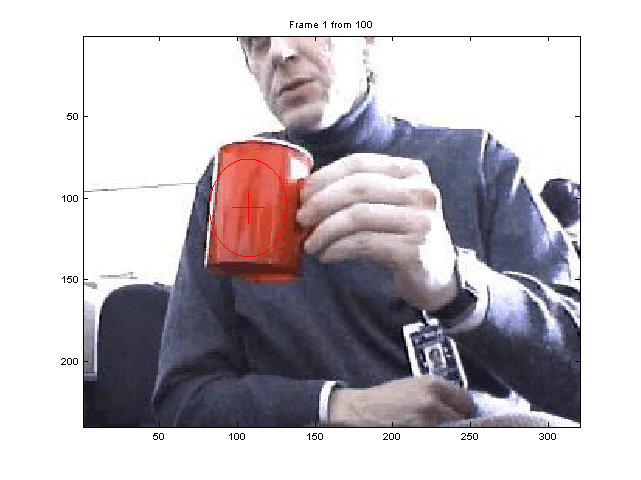
\includegraphics[width=\textwidth]{results/redcup/Frame0001.png}
         \end{subfigure}%
         \begin{subfigure}[b]{0.4\textwidth}
                 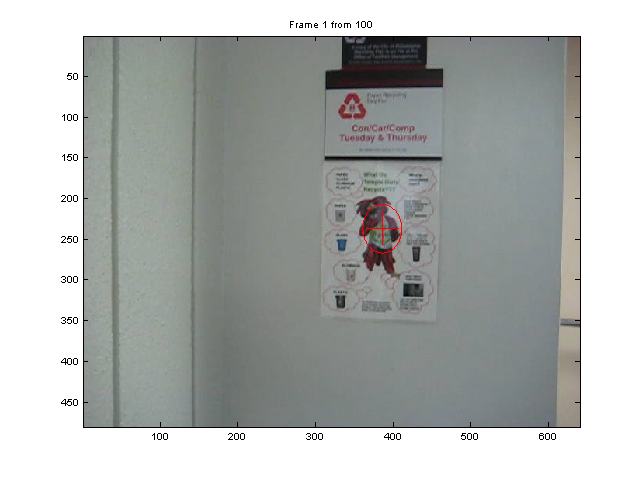
\includegraphics[width=\textwidth]{results/owl/Frame0001.png}
         \end{subfigure}
         \\
         \begin{subfigure}[b]{0.4\textwidth}
                 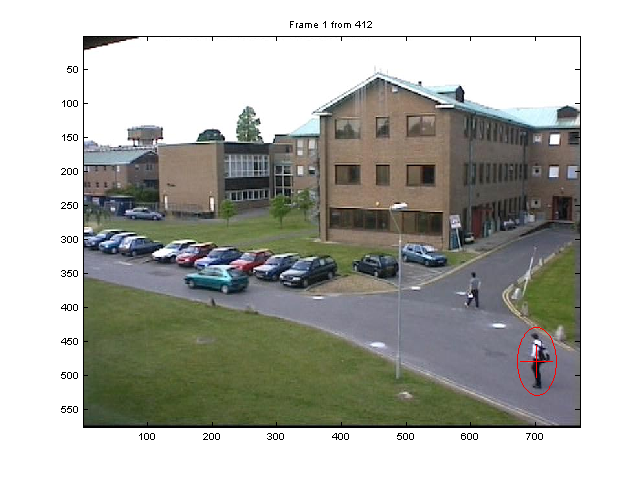
\includegraphics[width=\textwidth]{results/PETS01D1Human1man/Frame0001.png}
         \end{subfigure}
         \begin{subfigure}[b]{0.4\textwidth}
                  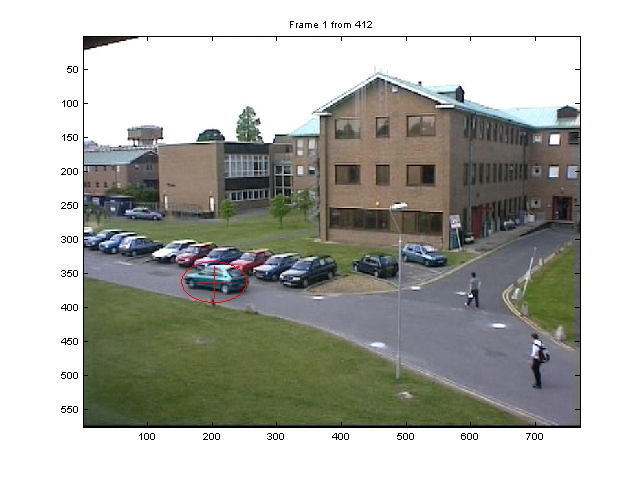
\includegraphics[width=\textwidth]{results/PETS01D1Human1car/Frame0001.png}
         \end{subfigure}
\end{figure}

\end{frame}

\begin{frame}
\frametitle{Red Cup}
\begin{figure}
         \centering
         \begin{subfigure}[b]{0.3\textwidth}
                 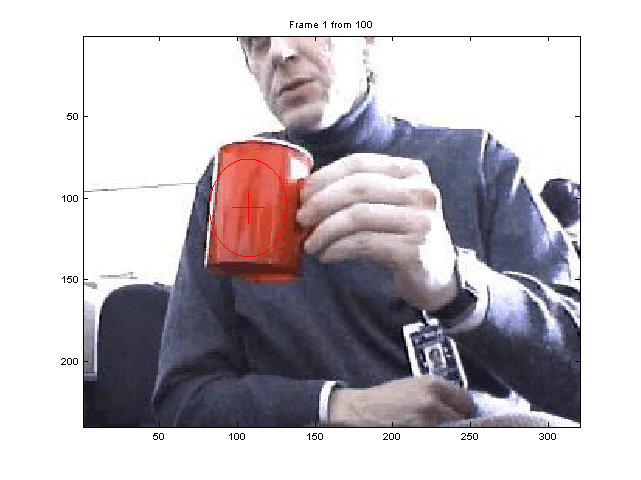
\includegraphics[width=\textwidth]{results/redcup/Frame0001.png}
         \end{subfigure}%
         \begin{subfigure}[b]{0.3\textwidth}
                 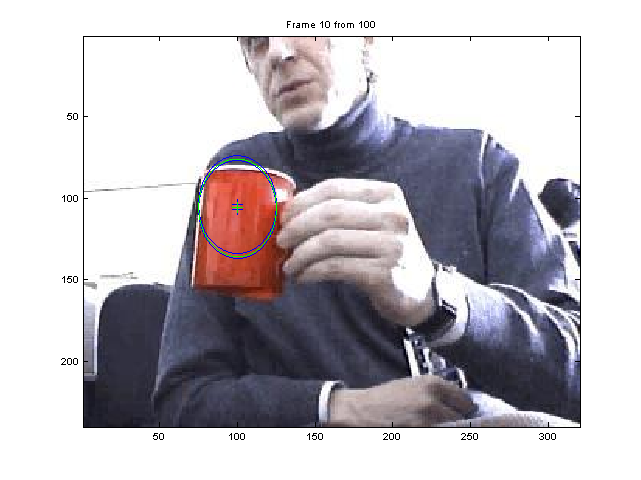
\includegraphics[width=\textwidth]{results/redcup/Frame0010.png}
         \end{subfigure}
         \begin{subfigure}[b]{0.3\textwidth}
                 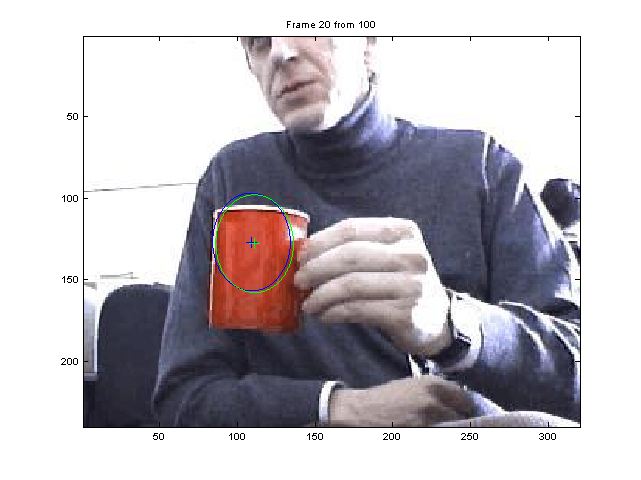
\includegraphics[width=\textwidth]{results/redcup/Frame0020.png}
         \end{subfigure}
         \\
         \begin{subfigure}[b]{0.3\textwidth}
                 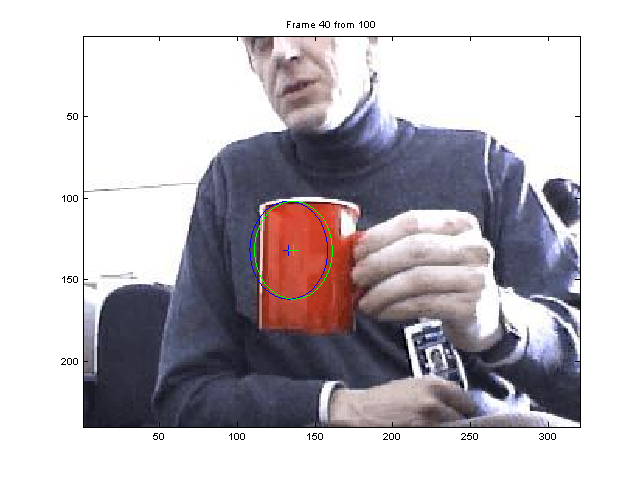
\includegraphics[width=\textwidth]{results/redcup/Frame0040.png}
         \end{subfigure}
         \begin{subfigure}[b]{0.3\textwidth}
                 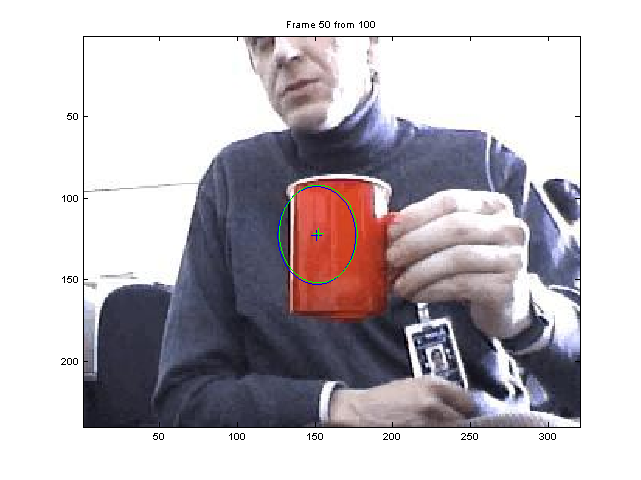
\includegraphics[width=\textwidth]{results/redcup/Frame0050.png}
         \end{subfigure}
         \begin{subfigure}[b]{0.3\textwidth}
                 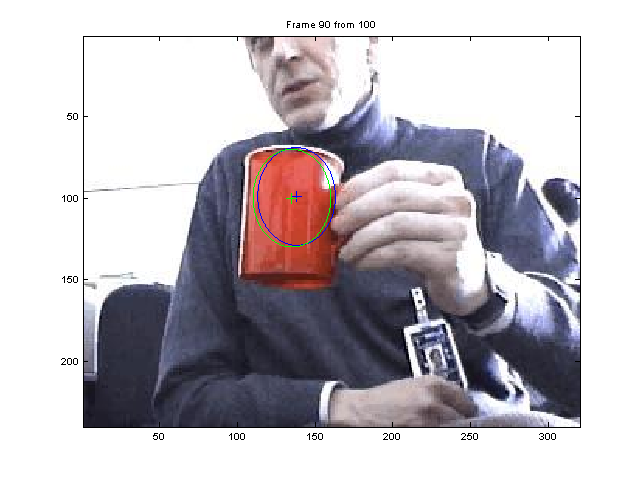
\includegraphics[width=\textwidth]{results/redcup/Frame0090.png}
         \end{subfigure}
\end{figure}         

\end{frame}

\begin{frame}
\frametitle{Owl}
\begin{figure}
         \centering
         \begin{subfigure}[b]{0.3\textwidth}
                 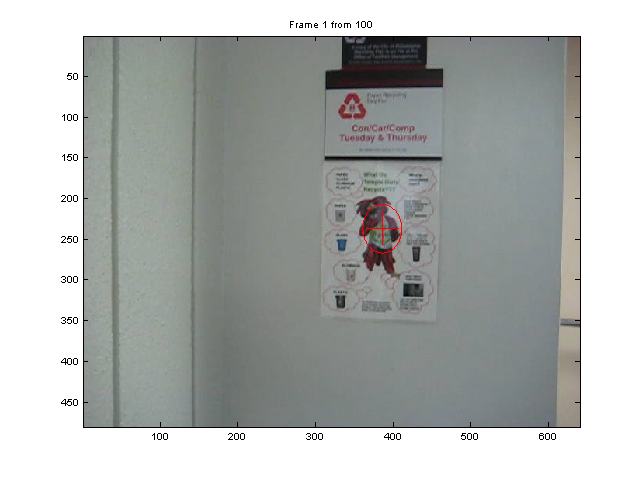
\includegraphics[width=\textwidth]{results/owl/Frame0001.png}
         \end{subfigure}%
         \begin{subfigure}[b]{0.3\textwidth}
                 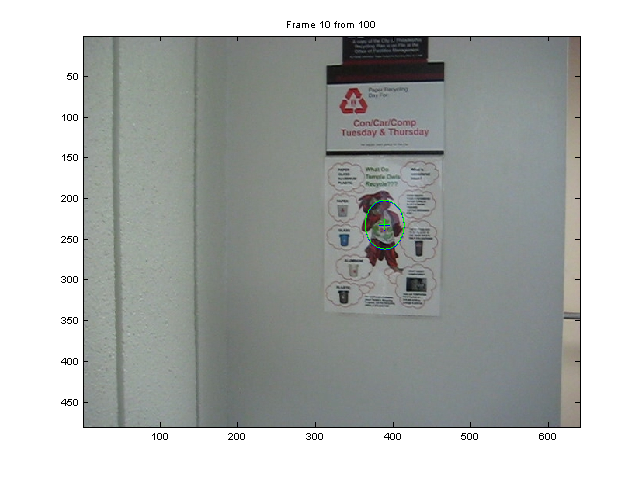
\includegraphics[width=\textwidth]{results/owl/Frame0010.png}
         \end{subfigure}
         \begin{subfigure}[b]{0.3\textwidth}
                 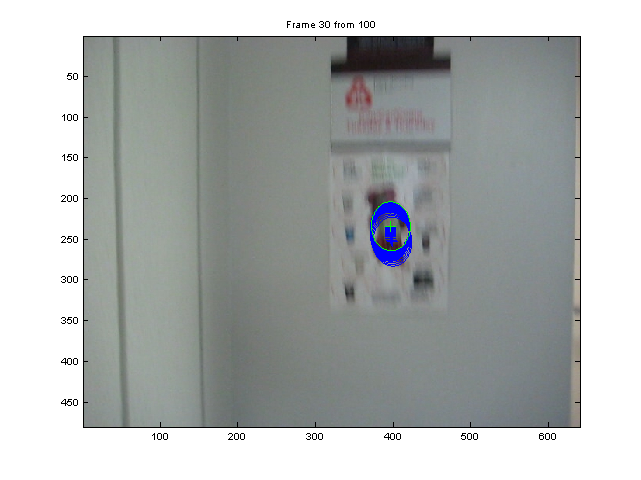
\includegraphics[width=\textwidth]{results/owl/Frame0030.png}
         \end{subfigure}
         \\
         \begin{subfigure}[b]{0.3\textwidth}
                 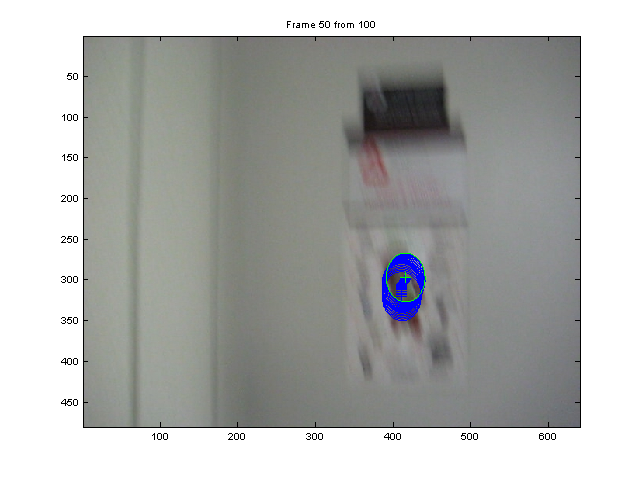
\includegraphics[width=\textwidth]{results/owl/Frame0050.png}
         \end{subfigure}
         \begin{subfigure}[b]{0.3\textwidth}
                 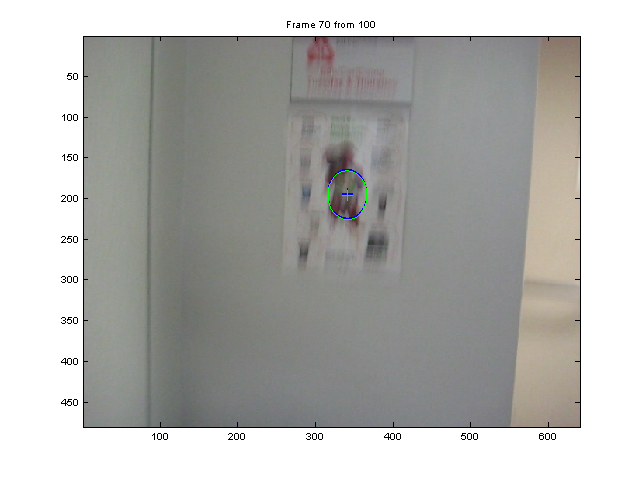
\includegraphics[width=\textwidth]{results/owl/Frame0070.png}
         \end{subfigure}
         \begin{subfigure}[b]{0.3\textwidth}
                 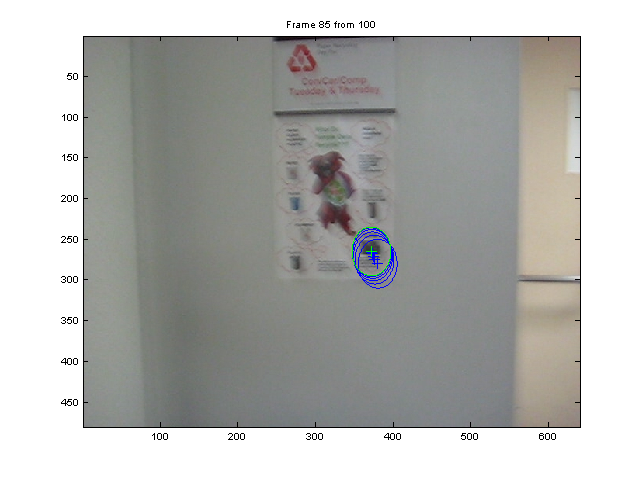
\includegraphics[width=\textwidth]{results/owl/Frame0085.png}
         \end{subfigure}
\end{figure}         

\end{frame}


\begin{frame}
\frametitle{PETS01D1Human1man}
\begin{figure}
         \centering
         \begin{subfigure}[b]{0.3\textwidth}
                 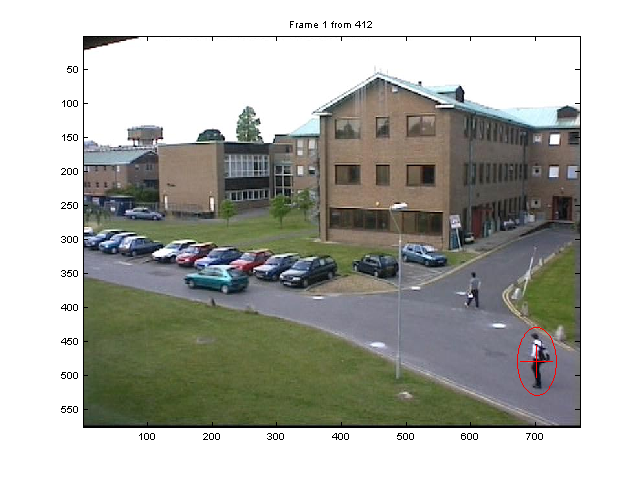
\includegraphics[width=\textwidth]{results/PETS01D1Human1man/Frame0001.png}
         \end{subfigure}%
         \begin{subfigure}[b]{0.3\textwidth}
                 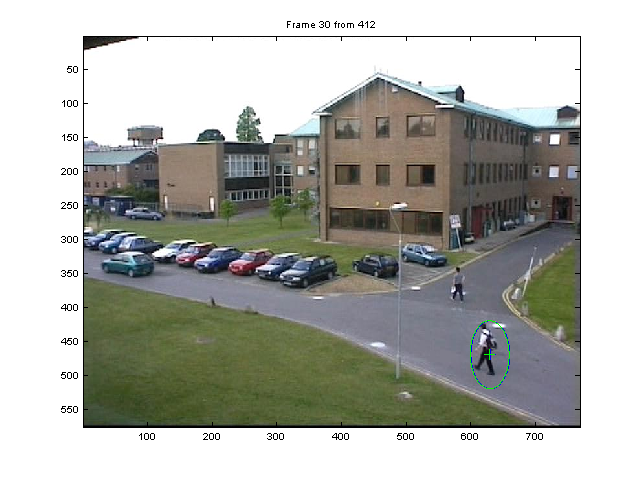
\includegraphics[width=\textwidth]{results/PETS01D1Human1man/Frame0030.png}
         \end{subfigure}
         \begin{subfigure}[b]{0.3\textwidth}
                 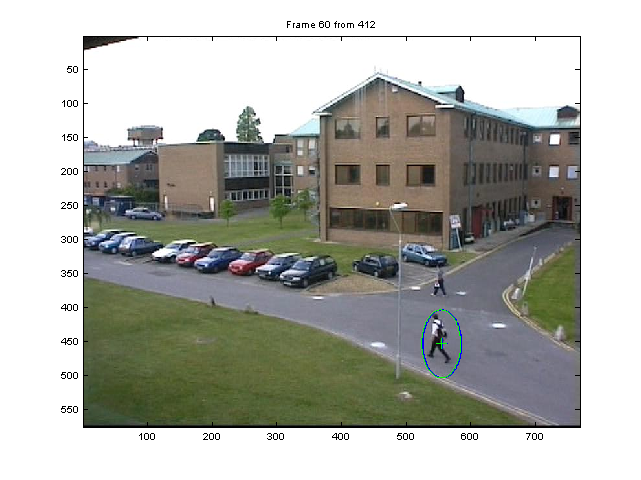
\includegraphics[width=\textwidth]{results/PETS01D1Human1man/Frame0060.png}
         \end{subfigure}
         \\
         \begin{subfigure}[b]{0.3\textwidth}
                 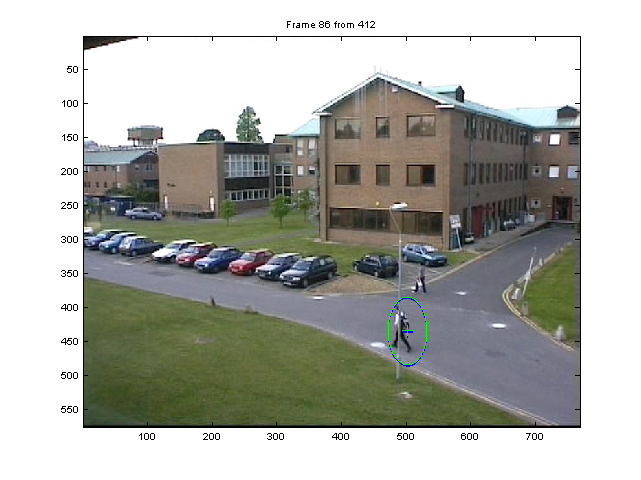
\includegraphics[width=\textwidth]{results/PETS01D1Human1man/Frame0086.png}
         \end{subfigure}
         \begin{subfigure}[b]{0.3\textwidth}
                 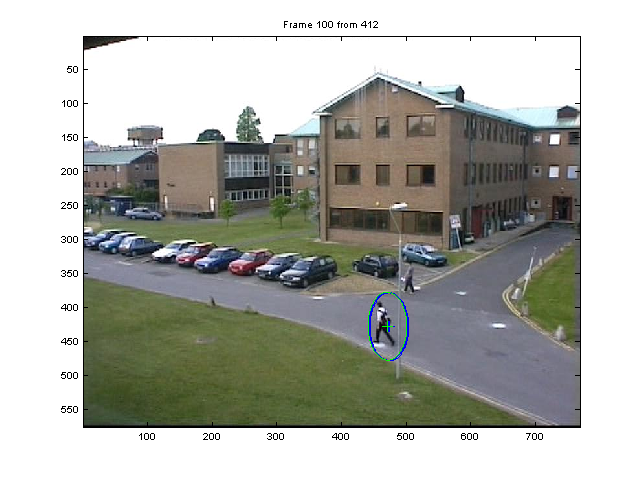
\includegraphics[width=\textwidth]{results/PETS01D1Human1man/Frame0100.png}
         \end{subfigure}
         \begin{subfigure}[b]{0.3\textwidth}
                 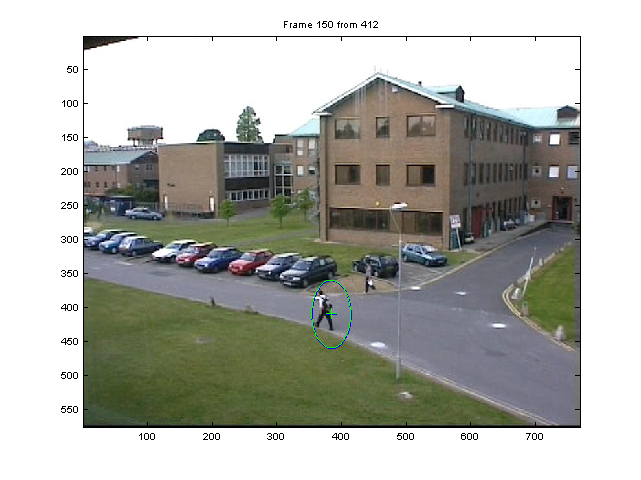
\includegraphics[width=\textwidth]{results/PETS01D1Human1man/Frame0150.png}
         \end{subfigure}
\end{figure}         

\end{frame}

\begin{frame}
\frametitle{PETS01D1Human1car}
\begin{figure}
         \centering
         \begin{subfigure}[b]{0.3\textwidth}
                 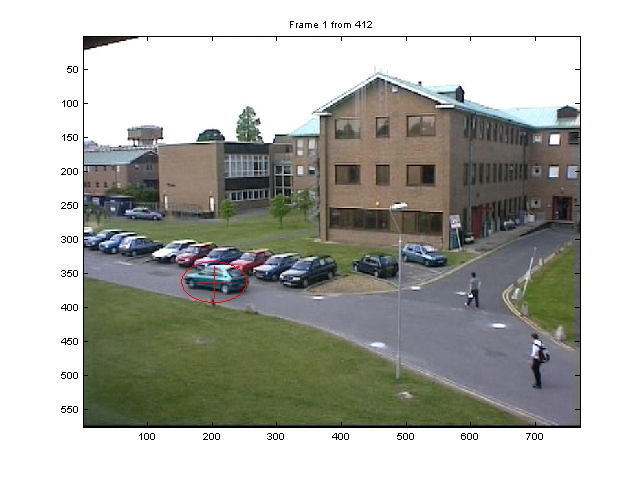
\includegraphics[width=\textwidth]{results/PETS01D1Human1car/Frame0001.png}
         \end{subfigure}%
         \begin{subfigure}[b]{0.3\textwidth}
                 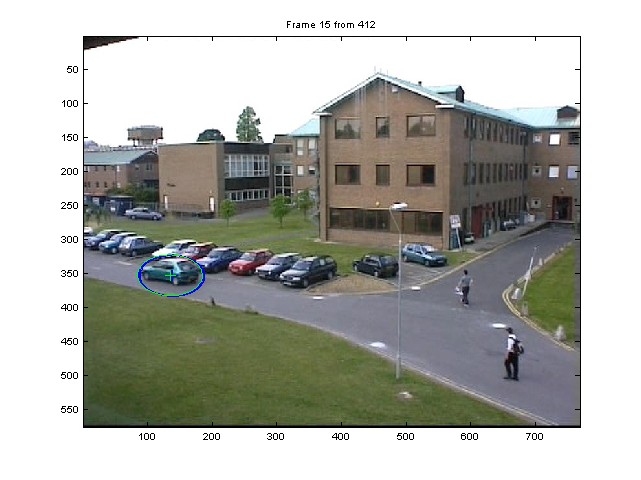
\includegraphics[width=\textwidth]{results/PETS01D1Human1car/Frame0015.png}
         \end{subfigure}
         \begin{subfigure}[b]{0.3\textwidth}
                 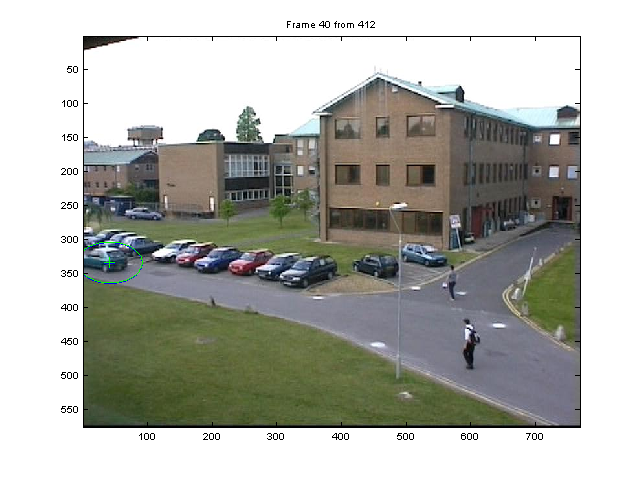
\includegraphics[width=\textwidth]{results/PETS01D1Human1car/Frame0040.png}
         \end{subfigure}
         \\
         \begin{subfigure}[b]{0.3\textwidth}
                 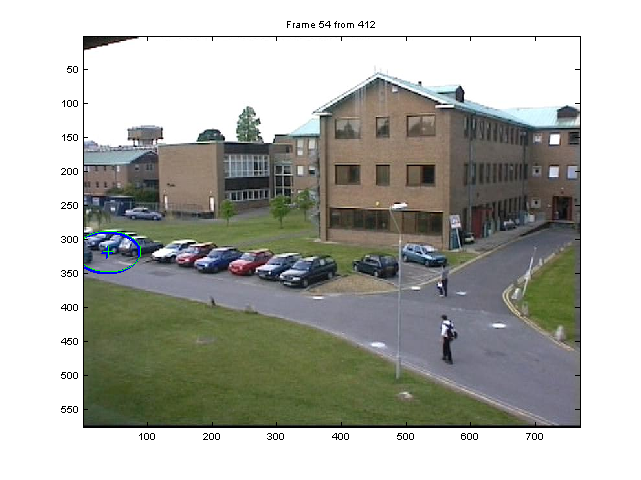
\includegraphics[width=\textwidth]{results/PETS01D1Human1car/Frame0054.png}
         \end{subfigure}
         \begin{subfigure}[b]{0.3\textwidth}
                 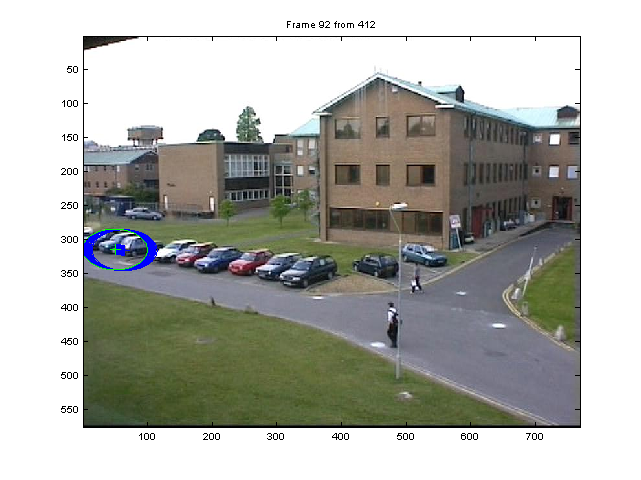
\includegraphics[width=\textwidth]{results/PETS01D1Human1car/Frame0092.png}
         \end{subfigure}
         \begin{subfigure}[b]{0.3\textwidth}
                 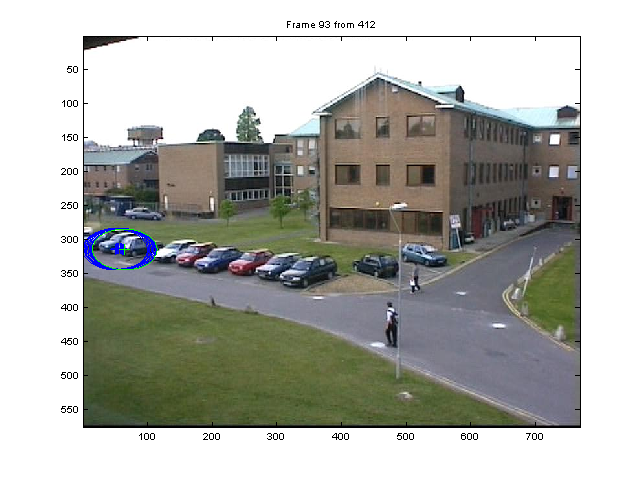
\includegraphics[width=\textwidth]{results/PETS01D1Human1car/Frame0093.png}
         \end{subfigure}
\end{figure}         

\end{frame}

%------------------------------------------------------------------------------%                                    References
\begin{frame}[allowframebreaks]
	\frametitle{References}
	\nocite{KernelBasedObjectTracking}
	\nocite{MeanShift}	
	\bibliographystyle{plain}
	\bibliography{bibliographie}
\end{frame}

%------------------------------------------------------------------------------%
\begin{frame}{The End}
\centering
\LARGE
\color{red}
 Thank you for your Attention!
 \nocite{BeamerTheme}
\end{frame}

\begin{frame}
\centering
\begin{figure}
	
\includegraphics{who.png}
\end{figure}
\end{frame}
\end{document}
